\section{Resultados}
\subsection{PCR em tempo real acomplado a High Resolution Melting Analysis}
As diferentes temperaturas de melt do DNA (Tm) podem ser extraídas dos dados
gerados no software High Resolution Melt v3.0.1 (Life Technologies). As curvas
alinhadas podem ser observadas na \cref{almeltc}.
\begin{wrapfigure}{r}{.5\textwidth}
        \centering
        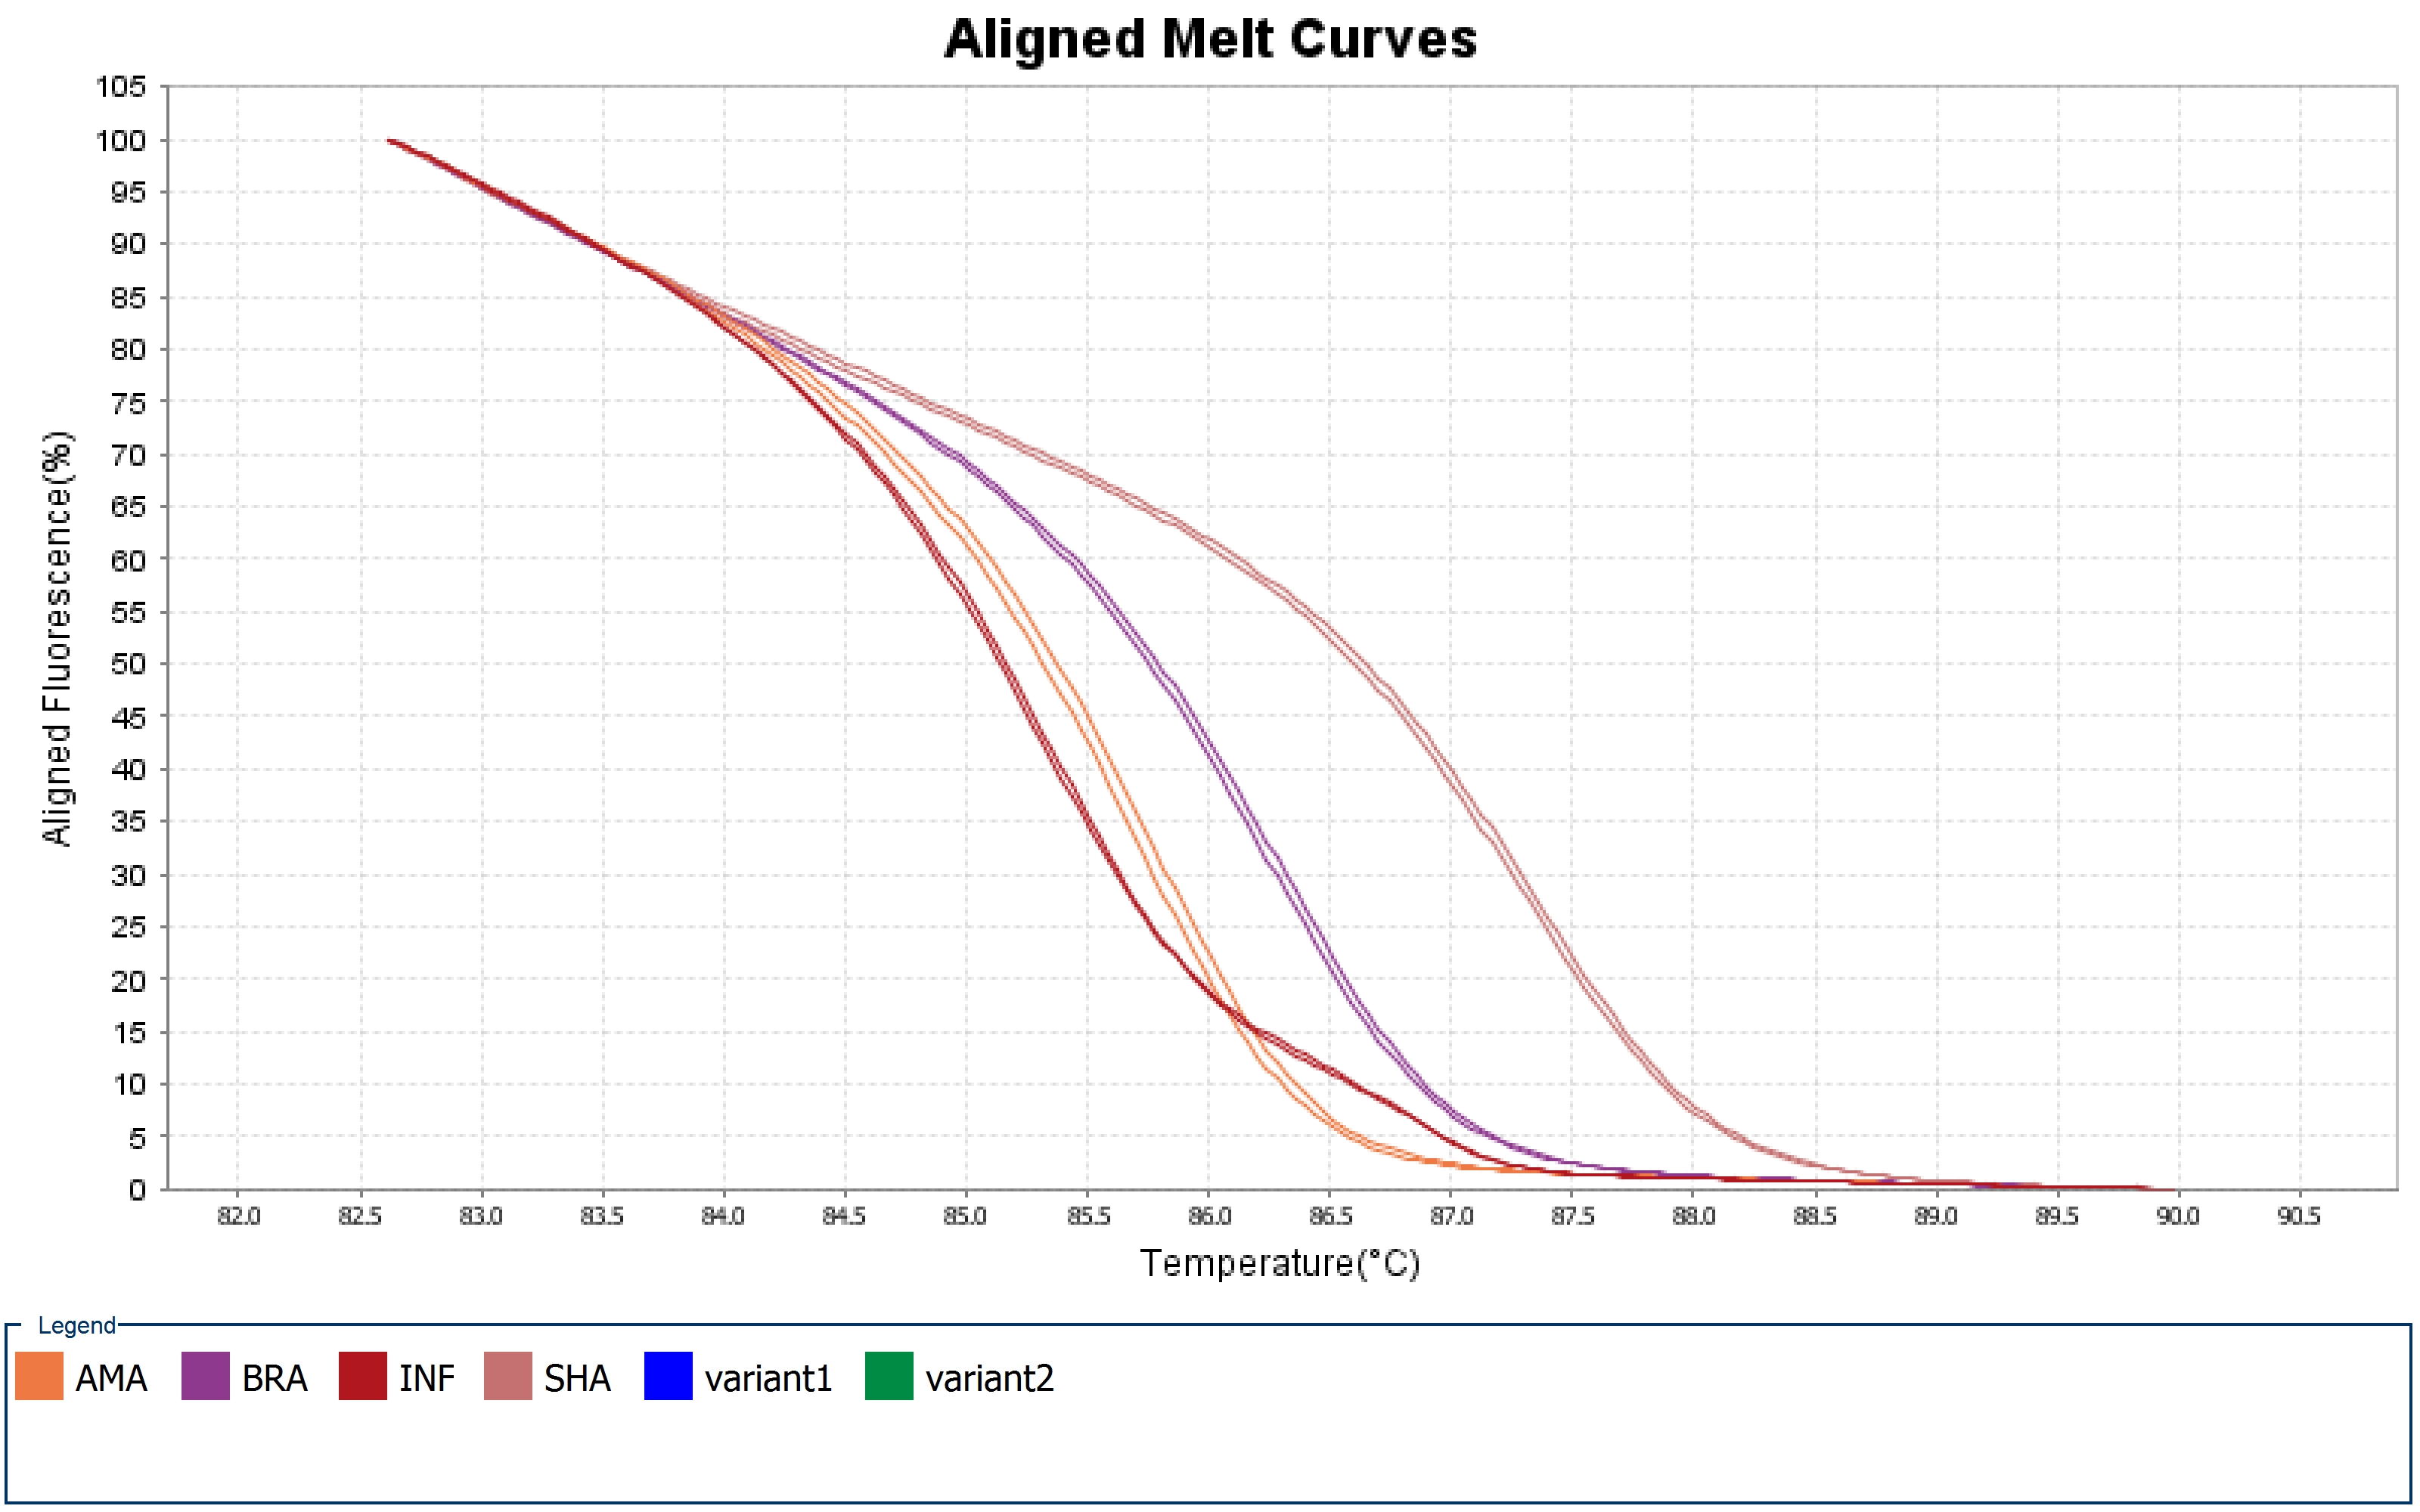
\includegraphics[width=.5\linewidth]{fig/Aligned Melt Curves.jpg}
        \caption{foto 1}
        \label{almeltc}
\end{wrapfigure}
    
\begin{wrapfigure}{r}{.5\textwidth}
        \centering
        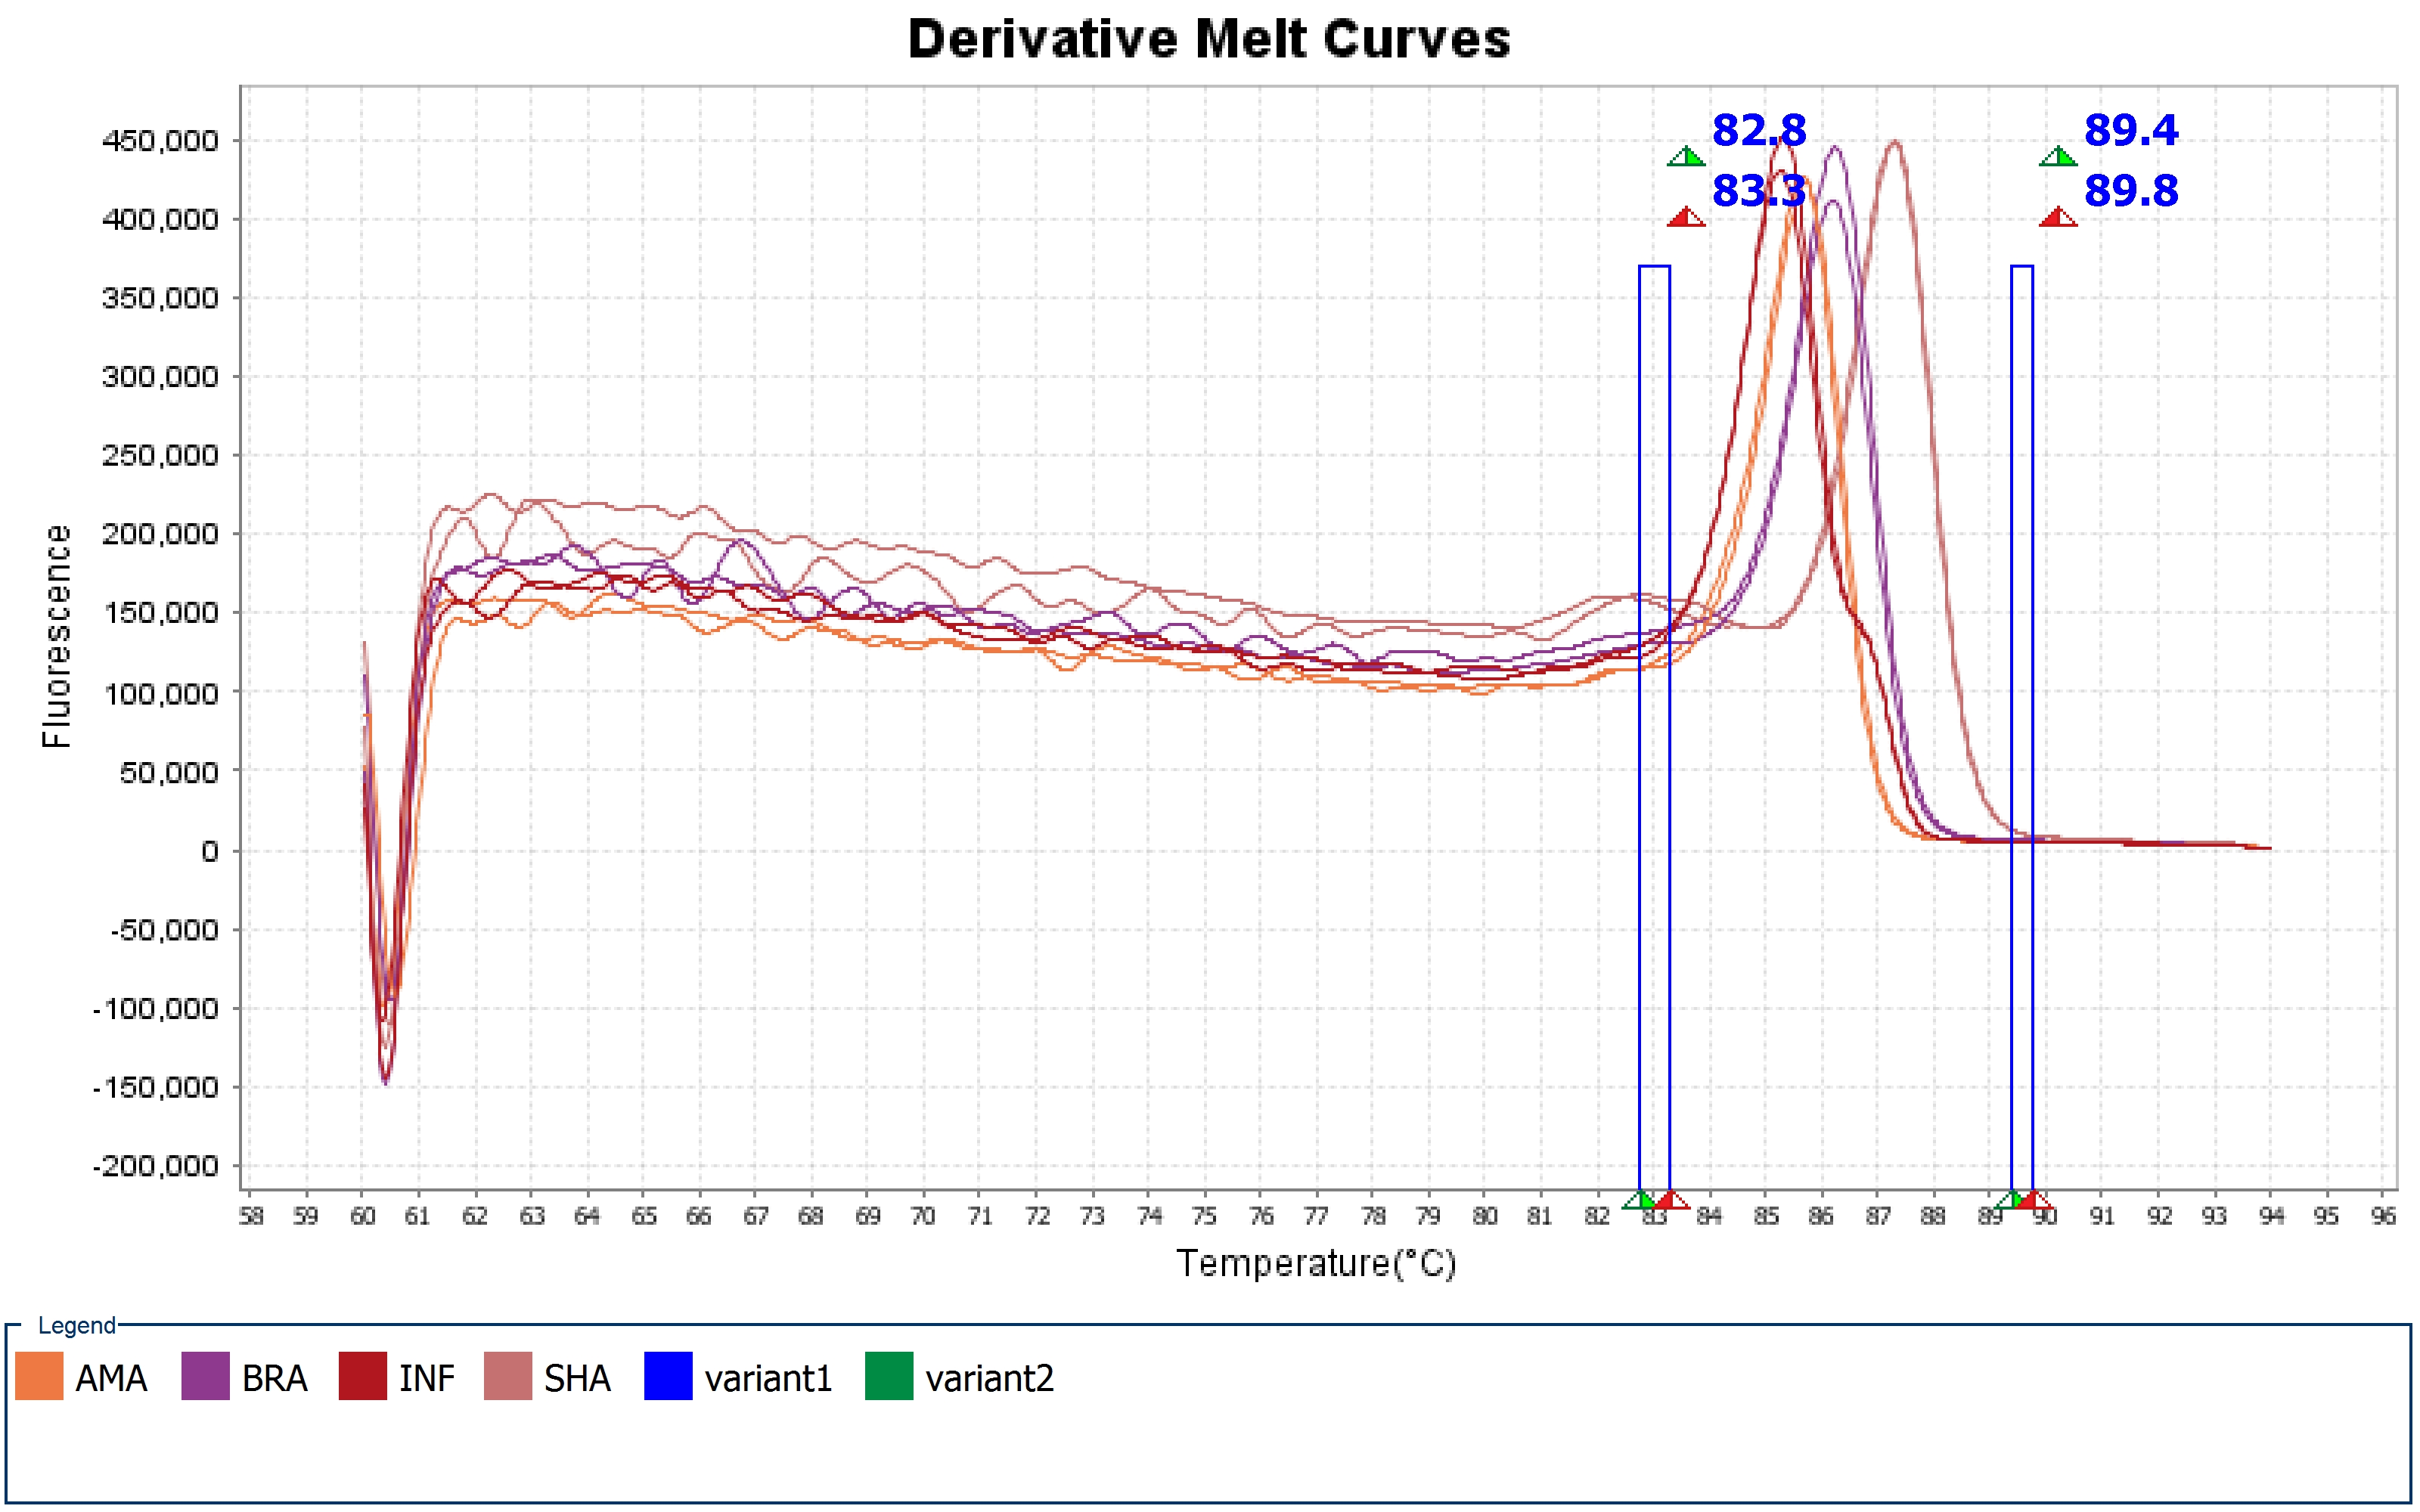
\includegraphics[width=.5\linewidth]{fig/Derivative Melt Curves.jpg}
        \caption{foto 1}
        \label{almeltc}
\end{wrapfigure}

\begin{wrapfigure}{r}{.5\textwidth}
        \centering
        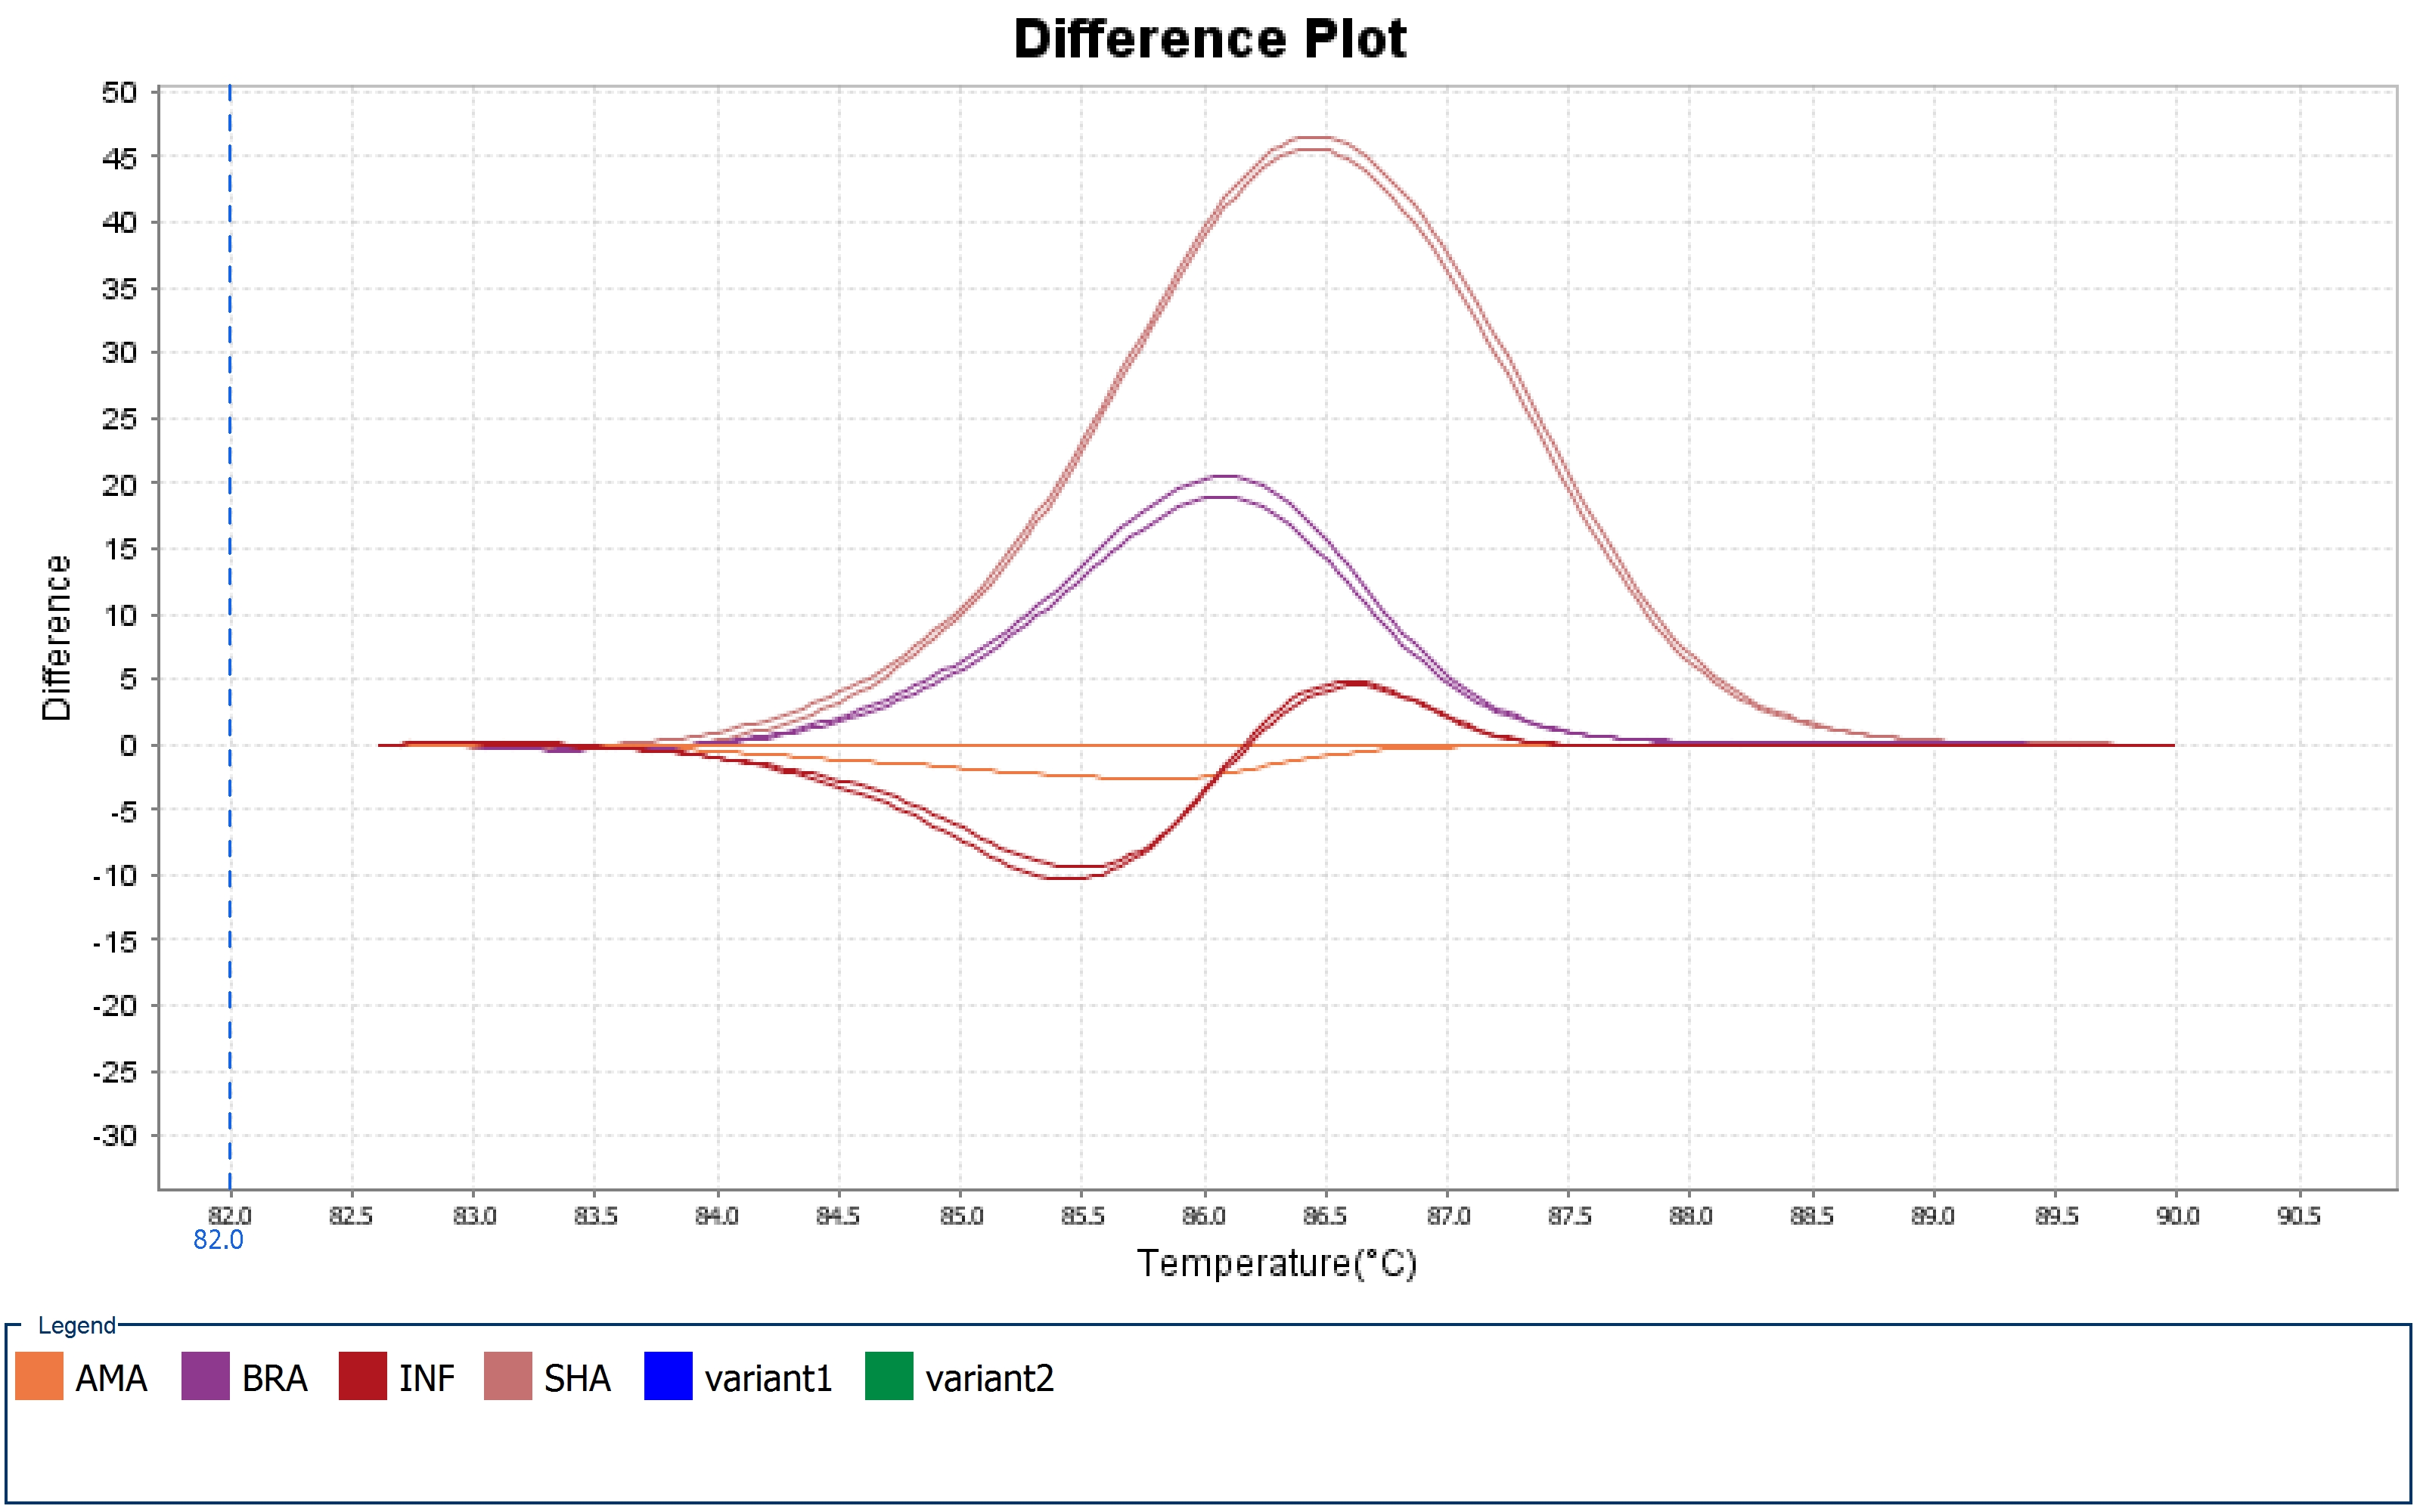
\includegraphics[width=.5\linewidth]{fig/Difference Plot.jpg}
        \caption{foto 1}
        \label{almeltc}
\end{wrapfigure}

\begin{wrapfigure}{r}{.5\textwidth}
        \centering
        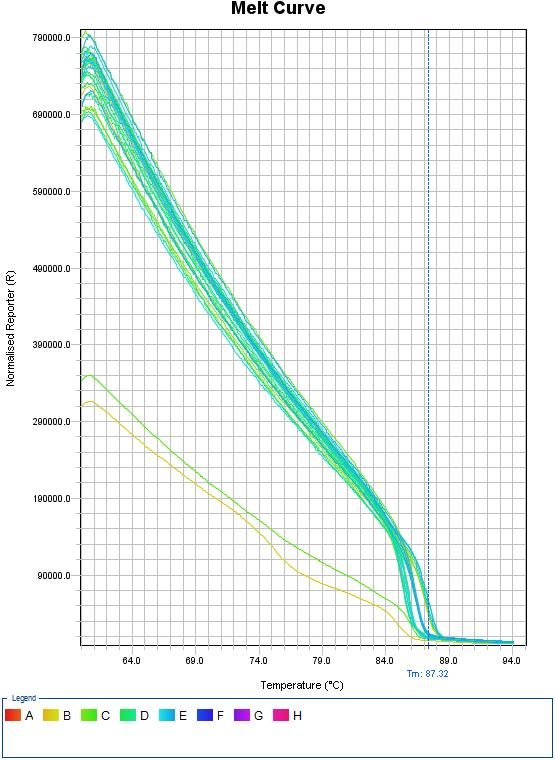
\includegraphics[width=.5\linewidth]{fig/Melt Curve.jpg}
        \caption{foto 1}
        \label{almeltc}
\end{wrapfigure}

\begin{wrapfigure}{r}{.5\textwidth}
        \centering
        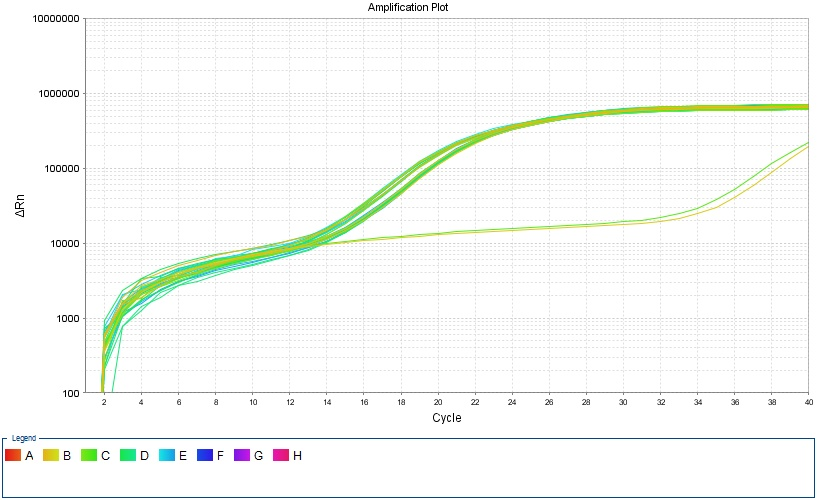
\includegraphics[width=.5\linewidth]{fig/Amplification Plot.jpg}
        \caption{foto 1}
        \label{almeltc}
\end{wrapfigure}


